\usetikzlibrary{circuits.ee.IEC}

\tikzset{circuit declare symbol = AC source}
\tikzset{AC source IEC graphic/.style={
    circuit symbol lines,
    circuit symbol size=width 2 height 2,
    shape=generic circle IEC,
    /pgf/generic circle IEC/before background={
    \pgfpathmoveto{\pgfpoint{-0.8pt}{0pt}}
    \pgfpathsine{\pgfpoint{0.4pt}{0.4pt}}
    \pgfpathcosine{\pgfpoint{0.4pt}{-0.4pt}}
    \pgfpathsine{\pgfpoint{0.4pt}{-0.4pt}}
    \pgfpathcosine{\pgfpoint{0.4pt}{0.4pt}}
    \pgfusepath{stroke}
    },
    transform shape, draw
  }
}
\tikzset{circuit ee IEC/.append style=
  {set AC source graphic = AC source IEC graphic}
}

\begin{figure}
   \centering
   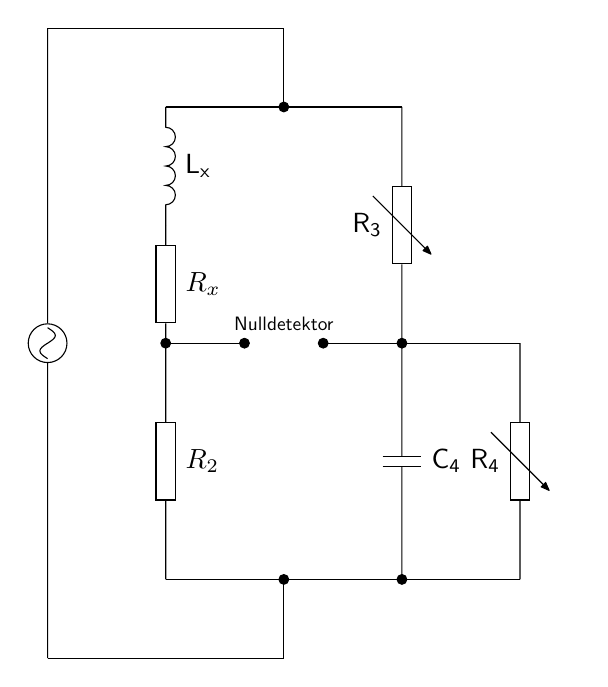
\begin{tikzpicture}[circuit ee IEC, font=\sffamily]
   \draw (0,0) to [AC source](0,-8);
   \draw (0,0) -- (3,0);
   \draw (3,0) -- (3, -1);
   \node[contact] at (3,-1) {};
   \draw (1.5, -1) -- (4.5, -1);
   \draw (1.5,-1) to [inductor={info={L$\mathsf{_{x}}$},info'={$\mathsf{_{}}$}}] (1.5,-2.5);
   \draw (1.5, -2.5) to [resistor={info={$R_x$}}] (1.5, -4);
   \draw (1.5, -4) to [resistor={info={$R_2$}}] (1.5, -7);
   \draw (4.5, -1) to  [resistor={adjustable={info={$\mathsf{_{}}$}}, info'={R$\mathsf{_{3}}$}}] (4.5,-4);
   \node[scale=0.7] at (3,-3.75) {Nulldetektor};
   \node[contact] at (1.5,-4) {};
   \node[contact] at (2.5, -4) {};
   \node[contact] at (3.5, -4) {};
   \node[contact] at (4.5, -4) {};
   \draw (1.5, -4) -- (2.5, -4);
   \draw (3.5, -4) -- (4.5, -4);
   \draw (1.5, -7) -- (4.5, -7);
   \node[contact] at (3,-7) {};
   \draw (4.5,-4) to [capacitor={info={C$\mathsf{_{4}}$},info'={$\mathsf{_{}}$}}] (4.5,-7);
   \node[contact] at (4.5, -7) {};
   \draw (6, -4) to  [resistor={adjustable={info={$\mathsf{_{}}$}}, info'={R$\mathsf{_{4}}$}}] (6,-7);
   \draw (4.5, -7) -- (6,-7);
   \draw (4.5, -4) -- (6,-4);
   \draw (0, -8) -- (3,-8);
   \draw (3, -8) -- (3,-7);
   \end{tikzpicture}
   \caption{Induktivitätsmessbrücke}
   % \label{fig:Induktivitätsmessbrücke}
\end{figure}
